\documentclass[fleqn]{jbook}
\usepackage{physpub}

\begin{document}

\begin{question}{専攻 問題4}{}

電磁波は光速で伝わる波でありながら、粒子(光子)としても振る舞う。波長
(またはエネルギー)帯によって、電磁波はいくつかの異なる名前で呼ばれ、
またその検出法も異なる。

\begin{subquestions}
\SubQuestion
  下の表にある A、B、Cそれぞれの電磁波(光子)について、対応する波長、
  周波数、エネルギーなどを求め、空欄を埋めた表を解答用紙に記せ。ただし、
  プランク定数は$h = 4 \times 10^{-15}\ \mathrm{eV \cdot sec}$、
  光速度は$c = 3 \times 10^{8}\ \mathrm{m / s}$とする。

  \begin{tabular}{|c|c|c|c|c|}
    \hline
      	&    波長 	&   周波数	&   エネルギー 	&     名称	\\
    \hline \hline
     A	& 		&   80\,MHz	& \hspace{25mm}	& \hspace{20mm}	\\
    \hline
     B 	&    500\,nm	& 		& 		&		\\
    \hline
     C 	& 		& 		&   100\,keV	&		\\
    \hline
  \end{tabular}

\SubQuestion
  上のB付近の周波数帯の光子を発生する現象を1つ挙げ、その基本過程を簡
  単に説明せよ。

\SubQuestion
  実験室に、Cのエネルギーを持った光子をランダムに発生する微弱な源がある。
  この光子を検出し、そのエネルギーを精度よく測定したい。この実験の全体の
  構成と、その中心となる検出器の原理を、図を用いて説明せよ。

\SubQuestion
  上の実験あるいは他の精密測定を行なおうとしたところ、同じ建物のどこか
  から来る、Aの付近の周波数を持った電磁波が、どうやらノイズとなって精
  密な測定を困難にしてるらしい。この電磁波の源をなるべく早くつきとめた
  い。物理系の実験室によくあるような装置、あるいは簡単に製作または借用
  できるような道具だてを使って、この電磁波の源がどこにあるか探し出すよ
  うな方法を考案し、説明せよ。複数の方法が考えられれば、それらを説明せ
  よ。

\SubQuestion
  この源をつきとめたところ、それを停止または撤去することは不可能とわか
  った。この状況でなお、目的とする精密測定を実験室で行なうには、どのよ
  うな対策を施せばよいか。具体的な方法と原理を説明せよ。

\SubQuestion
  \parbox[t]{90mm}{
 設問5で施した対策が効き、この電磁波からのノイズは抑えられた。そこで
 設問3の実験を再開したが、まだエネルギーの精密測定が困難であった。検
 出器からの信号をオッシロスコープで多数重ねて見たところ、図のスケッチ
 のように見えた。本来どのように見えるべきか、解答用紙にスケッチを示せ。
 またこの問題を引き起こしている原因として、どのようなものが考えられ、
 どんな対策がありうるか、列挙せよ。
}
\parbox[t]{60mm}{
%\vspace{60mm}
\begin{center}
  %% \includegraphics[clip]{1998phy4-0.eps}
  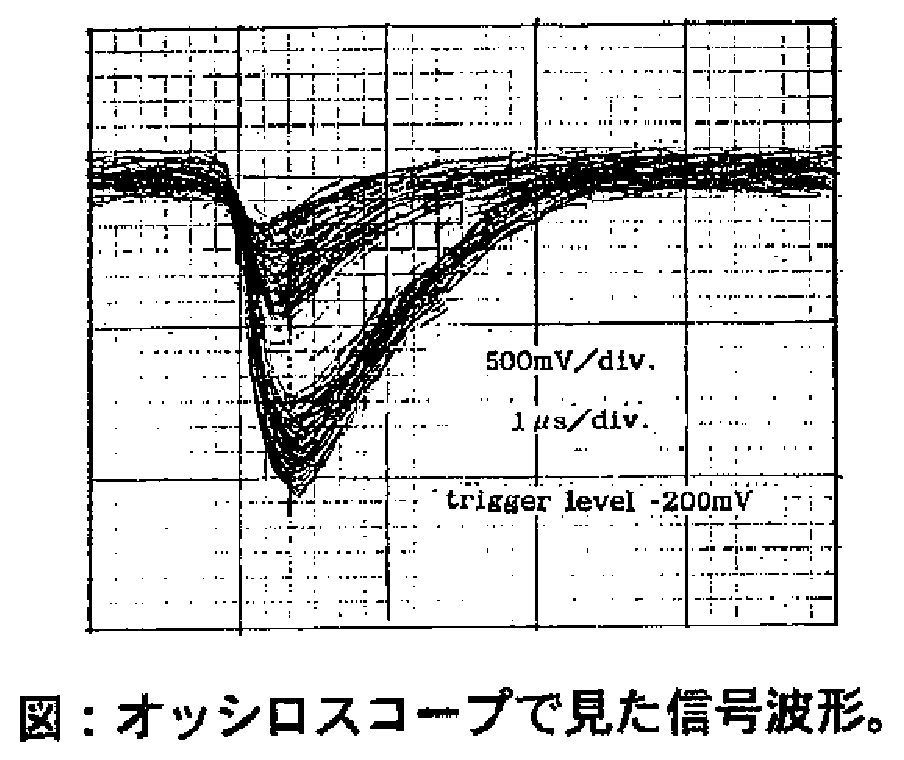
\includegraphics[width=60mm]{1998physQ4_0r.eps} %% KM, 重いので eps2 に変換
\end{center}
}
\end{subquestions}
\end{question}
\begin{answer}{専攻 問題4}{}

\begin{subanswers}
\SubAnswer

波長$\lambda$と周波数$\nu$とは、$c=\lambda\nu$の関係にある。
そして、エネルギー$E$は$E=h\nu$から計算できる。\\
\begin{center}
\begin{tabular}{|c|c|c|c|c|}
\hline
 &\bf{波長}&\bf{周波数}&\bf{エネルギー}&\bf{名称}\\
\hline
\hline
A&3.75\ [m]&80\ [MHz]%\footnote{TOKYO-FM}
&3.2$\times 10^{-7}$\ [eV]&超短波\\ \hline
B&500\ [nm]&600\ [THz]&2.4\ [eV]&可視光\\ \hline
C&12\ [pm]&2.5$\times 10^{19}$\ [Hz]&100\ [keV]&$\gamma$線\\ \hline
\end{tabular}
\end{center}

% added 28  Jul 2001 y.t.
[補足] Bは電波と書けば充分かもしれない。折角なので理科年表から国際電気通信条約無線規則による電波の名称を挙げておこう。

%\hbox{}\hskip-2cm
\begin{tabular}{c|lllllllllllllll}
波長[m]&$10^{-4}\sim$ &$10^{-3}\sim$ &$10^{-2}\sim$ &$0.1\sim$ &$1\sim$ &$10\sim$ &$100\sim$ &$10^{3}\sim$ &$10^{4}\sim$ &$10^{5}\sim$  \\ \hline
名称&サブミリ&ミリ&センチ&極超短&超短&短&中&長&超長\\
略号&&EHF&SHF&UHF&VHF&HF&MF&LF&VLF
\end{tabular}

UHF, VHF はテレビをアンテナに繋ぐときに良く聞くでしょ?
でもHって何の略なんだろ?

\SubAnswer
可視光を発する現象を挙げればよい。もちろんいろいろある。\\
 \begin{itemize}
 \item 白熱球 \\
      電流により加熱されたフィラメントの熱放射による発光。
 \item 蛍光灯 \\
      蛍光管中を流れる電子によって励起されたガスの蛍光により蛍光管の内側
      に塗られた蛍光体が励起されて起きる発光。フォトルミネッセンス
      の一つ。
 \item 発光ダイオード \\
      順バイアスで生じる、正孔と電子の結合によって励起状態になった原子が
      基底状態に戻るときの発光。エレクトロルミネッセンスの一つ。
 \item 可視光レーザー \\
       離散的な準位を持つ系で、周りからエネルギーを与え、電子を励起させる。
       励起した電子が低いエネルギー状態に移るとき、そのエネルギー差
       に相当する周波数の光を放出する。
  \item Naランプ \\
       ランプの中にNaなどの薄い蒸気を入れておく。ランプのフィラメントから
       発生する熱電子を電場を掛けて加速する。熱電子がある一定のエネルギー以
       上になってNa原子に当たると束縛電子が励起される。その電子が再
       び基底状態に落ちるときに可視光領域の光を放つ。
 \end{itemize}

\SubAnswer
計測したい電磁波は$\gamma$線であり、光源は微弱であり、しかも
そのエネルギーを精度よく測定したいから、NaIシンチレータなど
を用いるのがよい。
\begin{itemize}
\item NaIシンチレーターの原理\\
      NaIはNaの結晶に微量のTlを混入する。Tlがイオン化によって生じ
      た電子を捕え、その電子が励起状態から基底状態に落ちるときに発
      光する。
\item 実験の全体の構成\\
      シンチレーターでの発光を光電子増倍管に入れる。フォトカソー
      ドに当たった光子は10$\sim$20\%の効率で光電子を放出する。管内
      の電場で加速された光電子は第1段のダイノードに衝突し、入射電
      子1個に対して3$\sim$4個の電子を光電効果により叩き出す。以下、
      この過程を繰り返し、ダイノードが14個あるとすれば、最終的には
      だいたい$2\times 10^8$に増幅された電子パルスを得る。この電子
      パルスをAMPに通してADCに入力して、その出力をcomputerに入力す
      る。\\
      \begin{center}
       \leavevmode
%       
       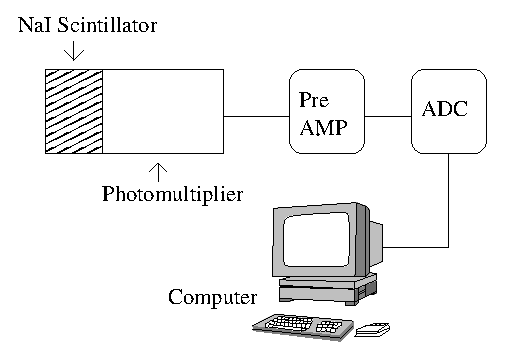
\includegraphics[clip]{1998phy4-1.eps}
      \end{center}
\end{itemize}

\SubAnswer
 いわゆる「電波」なのでアンテナを作ればよい。適当なコードやケー
 ブル、つまり電線をぐるぐる巻いてループアンテナを作るのがよい
 と思われる。波長が数メートルなので直径30cmぐらいで10回ぐらい
 巻けば十分実用性がある。ループアンテナだと軸方向に指向性があ
 るので電波源を探すのに都合が良い。アンテナからの出力は、ダイ
 オードで整流して電流計につなぐか、オシロスコープでみる。電波
 が微弱であるときは整流して平滑してオペアンプで増幅させれば良
 い。

\SubAnswer
 実験室を金属で覆い静電遮蔽すれば良い。電磁波の波長より短
 い金網で十分である。もしも、電波源が小さいのであればそれ自体
 を覆った方が楽である。実験室と同じ建物内といっているのだか
 ら、コンピュータであろうが、ノイズがテレビの電波であったりして、偏光
 方向が分かっているのなら、全てを覆わなくても、偏光方向に垂直
 になるように金属でスリットを作れば良い。テレビの電波は垂直に
 偏光しているので、波長よりも十分短い間隔で水平にスリットを作
 れば大体の電磁波は吸収できる。

\SubAnswer
 \parbox[t]{90mm}{
 信号の多い箇所が2つある。ピークの高い方が$\gamma$線の光電効果によ
 る吸収に相当し、低い方は主にコンプトン散乱で、後方散乱や自然
 放射線、除ききれなかったノイズもあるだろう。\\
 コンプトン散乱によるパルスを除くには、ディスクリミネーターを
 フォトマルとADCの間に入れると良い。ディスクリミネーターはス
 レッショルド以下の電圧の信号を除くので、スレッショルドの値を
 適切に調整すれば、光電効果によるパルスだけを取り出すことが可
 能である。光電ピークがぼけているのは$\gamma$線自体の広がり、
 およびフォトマルに掛る電圧が十分安定していないことによる。
 十分にウォームアップさせて回路を安定化させることが第一の対策
 である。
}
\parbox[t]{60mm}{
%\vspace{60mm}
\begin{center}
%% \includegraphics[clip]{1998phy4-2.eps}
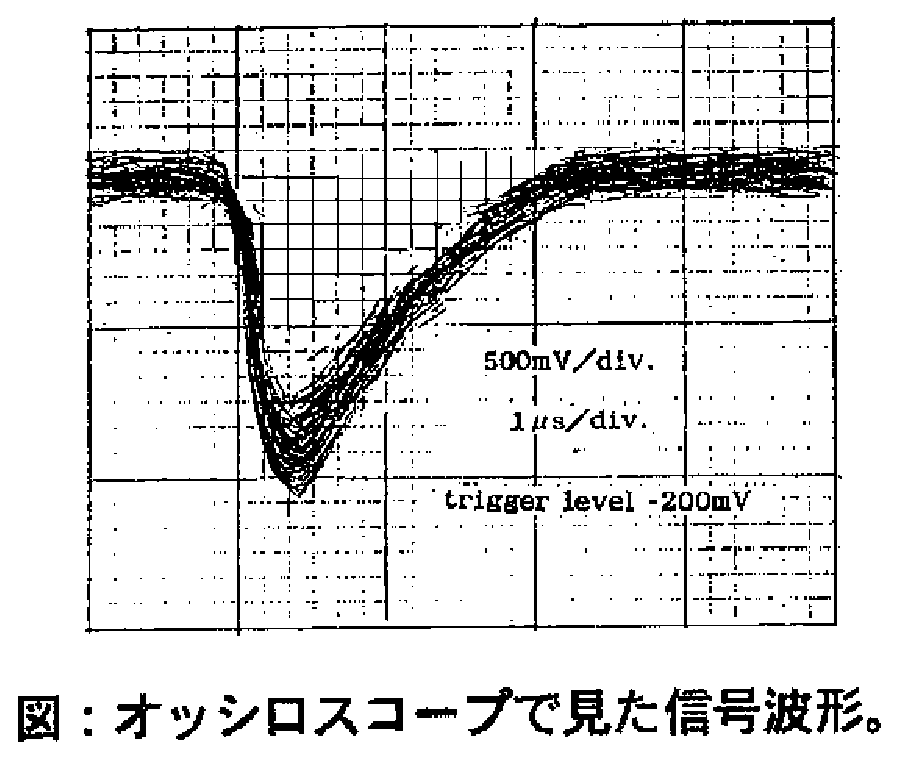
\includegraphics[width=60mm]{1998physQ4_2r.eps} %% KM, 重いので eps2 に変換
\end{center}
}

\end{subanswers}
\end{answer}


\end{document}
